% =====================================================================
\chapter{Sucesiones y series numéricas}
\label{tema:5}
% =====================================================================

Una serie es una suma de infinitos términos. Como no se pueden sumar infinitos números uno tras otro, la suma se define como el límite de las sumas parciales, y la primera pregunta es si ese límite existe. Este tema repasa los límites de sucesiones, estudia la serie geométrica y la serie armónica, que son los dos modelos de comparación fundamentales, y desarrolla los criterios de convergencia: comparación, cociente, raíz, integral y Leibniz. Se siguen los capítulos~22 y~23 de Spivak~\cite{spivak}, el capítulo~10 de Apostol~\cite{apostol}, las §5.1 a~5.6 de~\cite{openstax2}, las §10.1 a~10.3 de Strang~\cite{strang} y las sesiones~94 y~95 del curso 18.01SC~\cite{mit1801}.

\section{Sucesiones}

\begin{definicion}[Límite de una sucesión]\label{def:limite-sucesion}
Una sucesión $(a_n)_{n\ge1}$ de números reales \emph{converge} a $\ell\in\R$, y se escribe $a_n\to\ell$ o $\lim_{n\to\infty}a_n=\ell$, si para cada $\varepsilon>0$ existe $N\in\N$ tal que $\abs{a_n-\ell}<\varepsilon$ para todo $n\ge N$. Se escribe $a_n\to\infty$ si para cada $M$ existe $N$ con $a_n>M$ para todo $n\ge N$. Una sucesión que no converge \emph{diverge}.
\end{definicion}

El límite, si existe, es único, y los límites de sucesiones cumplen las mismas reglas algebraicas que los de funciones (módulo~0.5): el límite de una suma, de un producto o de un cociente con denominador de límite no nulo es la suma, el producto o el cociente de los límites. También vale el criterio del encaje: si $a_n\le b_n\le c_n$ y $a_n,c_n\to\ell$, entonces $b_n\to\ell$. Si $a_n=f(n)$ y $f(x)\to\ell$ cuando $x\to\infty$, entonces $a_n\to\ell$, lo que permite usar la regla de L'Hôpital.

\begin{teorema}[Convergencia monótona]\label{teo:monotona-acotada}
Toda sucesión creciente y acotada superiormente converge a su supremo. Toda sucesión decreciente y acotada inferiormente converge a su ínfimo.
\end{teorema}

\begin{proof}
Sea $(a_n)$ creciente y acotada. Por el axioma del supremo de los números reales existe $\ell=\sup_n a_n$. Dado $\varepsilon>0$, $\ell-\varepsilon$ no es cota superior, luego existe $N$ con $a_N>\ell-\varepsilon$. Para $n\ge N$, por ser creciente, $\ell-\varepsilon<a_N\le a_n\le\ell$, es decir, $\abs{a_n-\ell}<\varepsilon$. El caso decreciente se obtiene aplicando lo anterior a $(-a_n)$.
\end{proof}

\begin{ejemplo}[Potencias]\label{ej:potencias}
Si $\abs{r}<1$, entonces $r^{n}\to0$. Para $r=0$ es evidente. Si $0<\abs{r}<1$, se escribe $\frac{1}{\abs r}=1+h$ con $h>0$; por la desigualdad de Bernoulli (módulo~0.1), $(1+h)^{n}\ge1+nh$, luego $0<\abs{r}^{n}\le\frac{1}{1+nh}\to0$. Si $\abs r>1$, $\abs{r^{n}}\to\infty$; si $r=-1$, $r^{n}$ oscila entre $-1$ y~$1$ y no converge.
\end{ejemplo}

\section{Series numéricas}

\begin{definicion}[Serie]\label{def:serie}
Dada una sucesión $(a_n)_{n\ge1}$, su \emph{suma parcial} $n$-ésima es $S_n=a_1+\dots+a_n$. La serie $\sum_{n=1}^{\infty}a_n$ \emph{converge} si $(S_n)$ converge, y su \emph{suma} es $\sum_{n=1}^{\infty}a_n=\lim_{n\to\infty}S_n$. En otro caso la serie \emph{diverge}.
\end{definicion}

Si $\sum a_n$ y $\sum b_n$ convergen, también $\sum(\alpha a_n+\beta b_n)$, con suma $\alpha\sum a_n+\beta\sum b_n$, porque las sumas parciales se combinan del mismo modo. Suprimir o añadir un número finito de términos no cambia el carácter de la serie, aunque sí su suma.

\begin{teorema}[Serie geométrica]\label{teo:geometrica}
Sea $r\in\R$. La serie $\sum_{n=0}^{\infty}r^{n}$ converge si y solo si $\abs r<1$, y entonces
\[
\sum_{n=0}^{\infty}r^{n}=\frac{1}{1-r}.
\]
\end{teorema}

\begin{proof}
Si $r\neq1$, la suma geométrica finita (módulo~0.1) da $S_n=\sum_{k=0}^{n}r^{k}=\frac{1-r^{n+1}}{1-r}$. Si $\abs r<1$, $r^{n+1}\to0$ (\cref{ej:potencias}) y $S_n\to\frac{1}{1-r}$. Si $\abs r\ge1$, el término general $r^{n}$ no tiende a~$0$, y la serie diverge por la \cref{prop:condicion-necesaria}.
\end{proof}

\begin{proposicion}[Condición necesaria]\label{prop:condicion-necesaria}
Si $\sum a_n$ converge, entonces $a_n\to0$. Equivalentemente, si $a_n\not\to0$, la serie diverge.
\end{proposicion}

\begin{proof}
Si $S_n\to S$, también $S_{n-1}\to S$, y $a_n=S_n-S_{n-1}\to S-S=0$.
\end{proof}

La condición $a_n\to0$ es necesaria pero no suficiente, como muestra el resultado siguiente.

\begin{teorema}[La serie armónica diverge]\label{teo:armonica}
La serie $\sum_{n=1}^{\infty}\frac1n$ diverge; de hecho, $H_{2^{k}}\ge1+\frac k2$ para todo $k\in\N_0$.
\end{teorema}

\begin{proof}
Se agrupan los términos en bloques $\bigl[\frac{1}{2^{j-1}+1},\dots,\frac{1}{2^{j}}\bigr]$ para $j=1,\dots,k$. El bloque $j$ tiene $2^{j-1}$ términos, todos mayores o iguales que $\frac{1}{2^{j}}$, luego suma al menos $\frac12$. Por tanto $H_{2^{k}}\ge1+k\cdot\frac12$. Como $(H_n)$ es creciente y $H_{2^{k}}\to\infty$, $H_n\to\infty$.
\end{proof}

\begin{ejemplo}[Series telescópicas]\label{ej:telescopica}
Como $\frac{1}{k(k+1)}=\frac1k-\frac{1}{k+1}$, la suma parcial es $S_n=1-\frac{1}{n+1}$, y $\sum_{k=1}^{\infty}\frac{1}{k(k+1)}=1$. En general, si $a_k=b_k-b_{k+1}$, entonces $S_n=b_1-b_{n+1}$, y la serie converge si y solo si $(b_n)$ converge.
\end{ejemplo}

\section{Series de términos no negativos}

Si $a_n\ge0$ para todo $n$, las sumas parciales forman una sucesión creciente y, por el \cref{teo:monotona-acotada}, la serie converge si y solo si las sumas parciales están acotadas. De ahí salen todos los criterios de esta sección.

\begin{teorema}[Criterio de comparación]\label{teo:comparacion-series}
Sean $0\le a_n\le b_n$ para todo $n$. Si $\sum b_n$ converge, $\sum a_n$ converge y $\sum a_n\le\sum b_n$. Si $\sum a_n$ diverge, $\sum b_n$ diverge.
\end{teorema}

\begin{proof}
Las sumas parciales cumplen $\sum_{k=1}^{n}a_k\le\sum_{k=1}^{n}b_k\le\sum_{k=1}^{\infty}b_k$. Están acotadas y, por ser crecientes, convergen. La segunda afirmación es la contrarrecíproca.
\end{proof}

\begin{teorema}[Comparación en el límite]\label{teo:comparacion-limite-series}
Sean $a_n,b_n>0$ con $\frac{a_n}{b_n}\to L\in(0,\infty)$. Entonces $\sum a_n$ y $\sum b_n$ tienen el mismo carácter.
\end{teorema}

\begin{proof}
Existe $N$ tal que $\frac L2b_n\le a_n\le2L\,b_n$ para $n\ge N$. Si $\sum b_n$ converge, la desigualdad de la derecha y el \cref{teo:comparacion-series} dan la convergencia de $\sum_{n\ge N}a_n$; si $\sum a_n$ converge, la de la izquierda da la de $\sum b_n$. Los primeros $N-1$ términos no afectan al carácter.
\end{proof}

\begin{teorema}[Criterio de la integral]\label{teo:criterio-integral}
Sea $f\colon[1,\infty)\to\R$ positiva y decreciente y sea $a_k=f(k)$. Para todo $n\ge1$,
\[
\int_1^{n+1}f(x)\dif x\le\sum_{k=1}^{n}a_k\le a_1+\int_1^{n}f(x)\dif x .
\]
En consecuencia, $\sum a_k$ converge si y solo si $\int_1^{\infty}f$ converge.
\end{teorema}

\begin{proof}
$f$ es monótona, luego integrable en cada $[1,b]$ (\cref{teo:monotona}). Para $x\in[k,k+1]$, el decrecimiento da $f(k+1)\le f(x)\le f(k)$, y por la monotonía de la integral $a_{k+1}\le\int_k^{k+1}f\le a_k$. Sumando la desigualdad derecha para $k=1,\dots,n$ se obtiene $\int_1^{n+1}f\le\sum_{k=1}^{n}a_k$; sumando la izquierda para $k=1,\dots,n-1$, $\sum_{k=2}^{n}a_k\le\int_1^{n}f$. Si la integral converge, las sumas parciales están acotadas por $a_1+\int_1^{\infty}f$ y la serie converge; si diverge, $\int_1^{n+1}f\to\infty$ y la serie diverge.
\end{proof}

\begin{figure}[h]
\centering
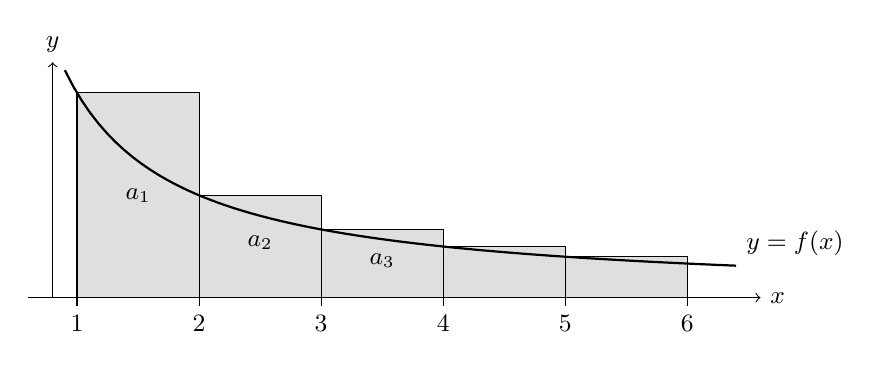
\begin{tikzpicture}[x=1.55cm,y=2.6cm,font=\small]
  \foreach \k in {1,...,5}{
    \pgfmathsetmacro{\h}{1/\k}
    \draw[fill=gray!25] (\k,0) rectangle ({\k+1},\h);
  }
  \draw[->] (0.6,0)--(6.6,0) node[right]{$x$};
  \draw[->] (0.8,0)--(0.8,1.15) node[above]{$y$};
  \draw[thick,domain=0.9:6.4,samples=80] plot (\x,{1/\x}) node[above right]{$y=f(x)$};
  \foreach \k in {1,...,6}{\draw (\k,0)--(\k,-0.04) node[below]{$\k$};}
  \node at (1.5,0.5) {$a_1$}; \node at (2.5,0.27) {$a_2$}; \node at (3.5,0.18) {$a_3$};
\end{tikzpicture}
\caption{Criterio de la integral con $f(x)=1/x$. El rectángulo sobre $[k,k+1]$ tiene altura $a_k=f(k)$ y contiene la región bajo la curva en ese intervalo; por eso $\sum_{k=1}^{n}a_k\ge\int_1^{n+1}f$. Desplazando los rectángulos una unidad a la izquierda quedan por debajo de la curva, y se obtiene la otra desigualdad.}
\label{fig:criterio-integral}
\end{figure}

\begin{corolario}[Series $p$]\label{cor:series-p}
La serie $\sum_{n=1}^{\infty}\frac{1}{n^{p}}$ converge si y solo si $p>1$. Además, $\ln(n+1)\le H_n\le1+\ln n$ para todo $n\in\N$.
\end{corolario}

\begin{proof}
Si $p\le0$, el término general no tiende a~$0$. Si $p>0$, $f(x)=x^{-p}$ es positiva y decreciente, y el \cref{teo:criterio-integral} con la \cref{prop:p-infinito} da el resultado. Con $p=1$, las desigualdades del teorema son $\ln(n+1)\le H_n\le1+\ln n$.
\end{proof}

Así, la serie armónica diverge, pero muy despacio: $H_{1000}$ está entre $\ln1001\approx6{,}91$ y $1+\ln1000\approx7{,}91$. En cambio, $\sum\frac{1}{n^{2}}$ converge, y su suma es menor que $1+\int_1^\infty x^{-2}\dif x=2$ (su valor exacto, $\frac{\pi^{2}}{6}\approx1{,}645$, se obtiene con otras técnicas).

\section{Criterios del cociente y de la raíz}

\begin{teorema}[Criterio del cociente]\label{teo:cociente}
Sea $a_n>0$ con $\frac{a_{n+1}}{a_n}\to L$. Si $L<1$, $\sum a_n$ converge; si $L>1$ (incluido $L=\infty$), diverge. Si $L=1$, el criterio no decide.
\end{teorema}

\begin{teorema}[Criterio de la raíz]\label{teo:raiz}
Sea $a_n\ge0$ con $\sqrt[n]{a_n}\to L$. Si $L<1$, $\sum a_n$ converge; si $L>1$, diverge. Si $L=1$, el criterio no decide.
\end{teorema}

\begin{proof}[Demostración del \cref{teo:raiz}]
Si $L<1$, sea $r$ con $L<r<1$. Existe $N$ con $\sqrt[n]{a_n}<r$, es decir, $a_n<r^{n}$, para $n\ge N$, y la serie converge por comparación con la geométrica de razón $r$. Si $L>1$, $\sqrt[n]{a_n}>1$, es decir, $a_n>1$, para $n$ grande, y el término general no tiende a~$0$.
\end{proof}

La demostración del criterio del cociente es análoga y se pide en el \cref{eje:5-cociente-dem}. Ambos criterios comparan con una serie geométrica, y por eso no deciden en el caso $L=1$: tanto $\sum\frac1n$, divergente, como $\sum\frac{1}{n^{2}}$, convergente, tienen $L=1$. Son especialmente útiles con factoriales y potencias $n$-ésimas.

\begin{ejemplo}\label{ej:cociente}
Para $a_n=\frac{n^{2}}{2^{n}}$, $\frac{a_{n+1}}{a_n}=\frac{(n+1)^{2}}{2n^{2}}\to\frac12<1$, y la serie converge. Para $a_n=\frac{x^{n}}{n!}$ con $x>0$, $\frac{a_{n+1}}{a_n}=\frac{x}{n+1}\to0$, y la serie converge para todo $x>0$; en el \cref{tema:6} se verá que su suma es $e^{x}-1$ (sumando desde $n=1$).
\end{ejemplo}

\section{Series alternadas y convergencia absoluta}

\begin{definicion}[Convergencia absoluta y condicional]\label{def:absoluta}
La serie $\sum a_n$ converge \emph{absolutamente} si $\sum\abs{a_n}$ converge. Si $\sum a_n$ converge pero $\sum\abs{a_n}$ diverge, converge \emph{condicionalmente}.
\end{definicion}

\begin{teorema}\label{teo:absoluta-series}
Toda serie absolutamente convergente es convergente, y $\bigl|\sum a_n\bigr|\le\sum\abs{a_n}$.
\end{teorema}

\begin{proof}
Se cumple $0\le a_n+\abs{a_n}\le2\abs{a_n}$, luego $\sum(a_n+\abs{a_n})$ converge por comparación, y $\sum a_n=\sum(a_n+\abs{a_n})-\sum\abs{a_n}$ es diferencia de dos series convergentes. La desigualdad se obtiene en el límite de $\bigl|\sum_{k\le n}a_k\bigr|\le\sum_{k\le n}\abs{a_k}$.
\end{proof}

\begin{teorema}[Criterio de Leibniz]\label{teo:leibniz}
Sea $(b_n)$ decreciente con $b_n\to0$ (luego $b_n\ge0$). La serie alternada $\sum_{n=1}^{\infty}(-1)^{n+1}b_n=b_1-b_2+b_3-\cdots$ converge, y su suma $S$ cumple $\abs{S-S_n}\le b_{n+1}$ para todo $n$.
\end{teorema}

\begin{proof}
Las sumas parciales pares cumplen $S_{2n+2}=S_{2n}+(b_{2n+1}-b_{2n+2})\ge S_{2n}$, luego son crecientes. Las impares cumplen $S_{2n+1}=S_{2n-1}-(b_{2n}-b_{2n+1})\le S_{2n-1}$, luego son decrecientes. Además $S_{2n}=S_{2n-1}-b_{2n}\le S_{2n-1}\le S_1$, así que las pares están acotadas superiormente por $S_1$, y análogamente las impares están acotadas inferiormente por $S_2$. Por el \cref{teo:monotona-acotada}, $S_{2n}\to A$ y $S_{2n+1}\to B$, y $B-A=\lim(S_{2n+1}-S_{2n})=\lim b_{2n+1}=0$. Luego $S_n\to S=A=B$. Por último, $S$ está entre dos sumas parciales consecutivas cualesquiera $S_n$ y $S_{n+1}$, de modo que $\abs{S-S_n}\le\abs{S_{n+1}-S_n}=b_{n+1}$.
\end{proof}

\begin{ejemplo}[Serie armónica alternada]\label{ej:armonica-alternada}
La serie $1-\frac12+\frac13-\frac14+\cdots$ converge por el \cref{teo:leibniz}, pero no absolutamente (\cref{teo:armonica}): converge condicionalmente. En el \cref{tema:6} se demostrará que su suma es $\ln2$. Por la cota del error, $S_{999}$ aproxima $\ln2$ con error no mayor que $b_{1000}=10^{-3}$.
\end{ejemplo}

\begin{observacion}[Reordenaciones]
Una serie absolutamente convergente puede sumarse en cualquier orden con el mismo resultado. Con una serie condicionalmente convergente no ocurre así: un teorema de Riemann afirma que sus términos pueden reordenarse para obtener cualquier suma prefijada~\cite[cap.~23]{spivak}. El ejercicio~25 de la §10.3 de Strang~\cite{strang} muestra una reordenación de la serie armónica alternada cuya suma es $\frac12\ln2$.
\end{observacion}

\begin{observacion}[Errores frecuentes]\label{obs:5-errores}
(a) Deducir la convergencia de $a_n\to0$; la serie armónica es el contraejemplo. (b) Confundir la sucesión $(a_n)$ con la serie $\sum a_n$: $\frac{n}{n+1}\to1$, luego la sucesión converge y la serie diverge. (c) Aplicar el criterio de comparación o el de la integral a series con términos negativos, o el de la integral a una función no decreciente. (d) Concluir algo del criterio del cociente cuando $L=1$. (e) Olvidar que la fórmula de la serie geométrica empieza en $n=0$: $\sum_{n=1}^{\infty}r^{n}=\frac{r}{1-r}$.
\end{observacion}

\begin{observacion}[Conexión con el curso]
En el módulo~21, el retorno descontado $G_t=\sum_{k=0}^{\infty}\gamma^{k}R_{t+k+1}$ es una serie, y si $\abs{R}\le R_{\max}$ converge absolutamente por comparación con la geométrica, con $\abs{G_t}\le\frac{R_{\max}}{1-\gamma}$. En el módulo~7, la media exponencial de Adam con gradiente constante vale $(1-\beta^{k})g$, una suma geométrica finita, y las condiciones de Robbins--Monro sobre las tasas de aprendizaje, $\sum\eta_t=\infty$ y $\sum\eta_t^{2}<\infty$, las cumple $\eta_t=\frac1t$ precisamente por el \cref{cor:series-p}; las cotas $\sum_{t\le T}\frac1t\le1+\ln T$ que se usan allí son las del \cref{teo:criterio-integral}. En el módulo~6, la entropía de una distribución geométrica es la suma de la serie $\sum k\,2^{-k}$, que se calcula en el \cref{tema:6}.
\end{observacion}

\begin{lecturas}
\item Spivak~\cite{spivak}, cap.~22 «Infinite Sequences» y cap.~23 «Infinite Series».
\item Apostol~\cite{apostol}, cap.~10 «Sequences, Infinite Series, and Improper Integrals».
\item OpenStax~\cite{openstax2}, §5.1 «Sequences», §5.2 «Infinite Series», §5.3 «The Divergence and Integral Tests», §5.4 «Comparison Tests», §5.5 «Alternating Series» y §5.6 «Ratio and Root Tests».
\item Strang~\cite{strang}, §10.1 «The Geometric Series», §10.2 «Convergence Tests: Positive Series» y §10.3 «Convergence Tests: All Series».
\item MIT 18.01SC~\cite{mit1801}, unidad~5, parte~B, sesiones~94 «Infinite Series» y~95 «Series Comparison».
\end{lecturas}

\section*{Ejercicios del tema 5}
\addcontentsline{toc}{section}{Ejercicios del tema 5}

\begin{ejercicio}{1}{eje:5-vf}
Justifique si son verdaderas o falsas: (a) si $a_n\to0$, $\sum a_n$ converge; (b) si $\sum a_n$ converge, $a_n\to0$; (c) la sucesión $a_n=\ln\bigl(1+\frac1n\bigr)$ converge y la serie $\sum a_n$ también; (d) si $\sum\abs{a_n}$ converge, $\sum a_n$ converge; (e) si $\frac{a_{n+1}}{a_n}\to1$, la serie diverge.
\end{ejercicio}

\begin{ejercicio}{2}{eje:5-limites}
Calcule los límites: (a) $\frac{3n^{2}+1}{2n^{2}-n}$; (b) $\sqrt{n+1}-\sqrt{n}$; (c) $\frac{n}{2^{n}}$; (d) $\frac{\sin n}{n}$; (e) $\bigl(1+\frac2n\bigr)^{n}$ (puede usar que $\frac{\ln(1+x)}{x}\to1$ cuando $x\to0$).
\end{ejercicio}

\begin{ejercicio}{2}{eje:5-geometricas}
(a) Sume $\frac13+\frac19+\frac{1}{27}+\cdots$ y $1-\frac14+\frac{1}{16}-\cdots$. (b) Sume $\sum_{k=2}^{\infty}3\bigl(-\frac25\bigr)^{k}$. (c) Escriba $0{,}878787\ldots$ y $0{,}123123\ldots$ como series geométricas y como fracciones irreducibles.
\fuente{adaptado de Strang~\cite{strang}, §10.1, ejercicios 3 y~13.}
\end{ejercicio}

\begin{ejercicio}{2}{eje:5-pelota}
Una pelota se deja caer desde 10~m y, tras cada bote, sube hasta $\frac35$ de la altura desde la que cayó. Calcule la distancia vertical total que recorre. Si cada caída desde altura $h$ dura $\sqrt{2h/g}$, ¿es finito el tiempo total?
\fuente{adaptado de Strang~\cite{strang}, §10.1, ejercicio~2.}
\end{ejercicio}

\begin{ejercicio}{2}{eje:5-comparacion}
Estudie la convergencia por comparación directa o en el límite: (a) $\sum\frac{1}{n^{2}+10}$; (b) $\sum\frac{1}{2n-1}$; (c) $\sum\frac{n+1}{n^{3}+2}$; (d) $\sum\frac{1}{\sqrt{n^{2}+n}}$; (e) $\sum\sin\frac{1}{n^{2}}$.
\fuente{adaptado de Strang~\cite{strang}, §10.2, ejercicio~11.}
\end{ejercicio}

\begin{ejercicio}{2}{eje:5-cociente}
Estudie la convergencia con el criterio del cociente o de la raíz: (a) $\sum\frac{3^{n}}{n!}$; (b) $\sum\frac{n!}{n^{n}}$; (c) $\sum\frac{2^{n}}{n^{2}}$; (d) $\sum\bigl(\frac{n}{2n+1}\bigr)^{n}$; (e) $\sum\frac{1}{n^{3}}$ (¿qué ocurre?).
\fuente{adaptado de Strang~\cite{strang}, §10.2, ejercicios 21 y~28.}
\end{ejercicio}

\begin{ejercicio}{2}{eje:5-integral}
Use el criterio de la integral: (a) $\sum_{n\ge1}e^{-n}$ (compruebe sumándola como geométrica); (b) $\sum_{n\ge1}n\,e^{-n}$; (c) $\sum_{n\ge2}\frac{\ln n}{n}$; (d) $\sum_{n\ge2}\frac{1}{n(\ln n)^{2}}$.
\fuente{adaptado de Strang~\cite{strang}, §10.2, ejercicios 33, 34 y~38.}
\end{ejercicio}

\begin{ejercicio}{2}{eje:5-armonica}
(a) Con las cotas del \cref{cor:series-p}, demuestre que hacen falta más de 400 términos para que $H_n>7$, y que con $1097$ términos ya se supera. (b) Admitiendo que $H_n-\ln n$ decrece hacia la constante de Euler $\gamma\approx0{,}5772$, estime el primer $n$ con $H_n>7$.
\fuente{adaptado de Strang~\cite{strang}, §10.2, ejercicio~44.}
\end{ejercicio}

\begin{ejercicio}{2}{eje:5-alternadas}
Decida si convergen absolutamente, condicionalmente o no convergen: (a) $\sum\frac{(-1)^{n+1}}{n!}$; (b) $\sum\frac{(-1)^{n+1}3^{n}}{n!}$; (c) $\sum\frac{(-1)^{n+1}n^{2}}{1+n^{4}}$; (d) $\sum\frac{(-1)^{n}}{\sqrt n}$; (e) $\sum\frac{(-1)^{n}n}{n+1}$.
\fuente{adaptado de Strang~\cite{strang}, §10.3, ejercicios 3, 4 y~9.}
\end{ejercicio}

\begin{ejercicio}{2}{eje:5-error-alternada}
(a) Acote $\abs{S_5-\ln2}$ para la serie armónica alternada, sabiendo que su suma es $\ln2$, y compare con el error real. (b) ¿Cuántos términos de $\sum\frac{(-1)^{n+1}}{n^{2}}$ garantizan, por el \cref{teo:leibniz}, un error menor que $10^{-3}$?
\fuente{adaptado de Strang~\cite{strang}, §10.3, ejercicios 18 y~20.}
\end{ejercicio}

\begin{ejercicio}{2}{eje:5-descuento}
(a) Calcule el retorno descontado $G=\sum_{k=0}^{\infty}\gamma^{k}R_{k+1}$ con $\gamma=0{,}9$ si $R_k=1$ para todo $k$, y si $R_k=1$ solo para $k$ impar y $0$ para $k$ par. (b) En Adam, la media exponencial de un gradiente constante $g$ tras $k$ pasos es $(1-\beta^{k})g$. ¿Cuántos pasos hacen falta para que $1-\beta^{k}\ge0{,}99$ con $\beta=0{,}9$? ¿Y con $\beta=0{,}999$?
\end{ejercicio}

\begin{ejercicio}{3}{eje:5-armonica-dem}
(a) Demuestre que $H_{2n}-H_n\ge\frac12$ para todo $n\in\N$. (b) Deduzca, sin usar el \cref{teo:armonica}, que $(H_n)$ no está acotada. (c) Demuestre que si $\sum a_n$ converge, entonces $\sum_{k=n+1}^{2n}a_k\to0$, y obtenga una tercera prueba de la divergencia de la serie armónica.
\end{ejercicio}

\begin{ejercicio}{3}{eje:5-cociente-dem}
Demuestre el \cref{teo:cociente}. (Indicación: si $L<1$, fije $r\in(L,1)$ y pruebe por inducción que $a_{N+m}\le a_N\,r^{m}$ a partir de cierto $N$.)
\end{ejercicio}

\begin{ejercicio}{3}{eje:5-resto}
Sea $f$ positiva y decreciente en $[1,\infty)$ con $\int_1^{\infty}f$ convergente, y sea $R_n=\sum_{k=n+1}^{\infty}f(k)$ el resto de la serie. (a) Demuestre que $\int_{n+1}^{\infty}f\le R_n\le\int_n^{\infty}f$. (b) Para $f(x)=1/x^{2}$, deduzca que $\frac{1}{n+1}\le R_n\le\frac1n$ y estime $\sum_{k=1}^{\infty}\frac{1}{k^{2}}$ a partir de $S_{10}$, con una cota del error.
\end{ejercicio}

\begin{ejercicio}{3}{eje:5-euler}
Sea $c_n=H_n-\ln n$. Demuestre que $(c_n)$ es decreciente y que $c_n>0$ para todo $n$, y concluya que converge. (Indicación: $c_n-c_{n+1}=\int_n^{n+1}\frac{\dif x}{x}-\frac{1}{n+1}$.) Su límite es la constante de Euler, $\gamma\approx0{,}5772$.
\end{ejercicio}

\begin{ejercicio}{3}{eje:5-heron}
Sea $a_1=2$ y $a_{n+1}=\frac12\bigl(a_n+\frac{2}{a_n}\bigr)$. Demuestre que $a_n\ge\sqrt2$ para todo $n$ (use la desigualdad entre las medias aritmética y geométrica), que $(a_n)$ es decreciente y que converge a $\sqrt2$. Calcule $a_2$, $a_3$ y $a_4$ y compare con $\sqrt2$.
\end{ejercicio}
